\section{Evaluation Method}\label{Evaluation_Method}

In order to find our probing rate for run our experiments we worked with two testbeds we had access to. The first is a small setup in our office, the second is a testbed called Orbit Lab \cite{orbit2005}.

\subsection*{In-Office Lab}

The In-office lab was mainly used to work on finding the probing rate at which the test in Orbit lab testbed were going to be conducted. The setup at our office is primarily composed by the following components.

\begin{enumerate}
	\item Raspberry Pi 3 running Raspbian GNU/Linux 8 (Jessie)
	\item Wireless Access Point TP-Link AC1750
	\item Dell Laptop Inspiron running Ubuntu 16.04.4 LTS (Xenial Xerus)
\end{enumerate}

The wireless card driver on the Dell Laptop supported 802.11 a/b/g/n/ac. The driver is \textit{iwlwifi} version 4.4.0-130-generic and firmware=17.948900127.0. At the In-Office lab we setup our deployment as illustrated in figure \ref{image:In_Office_Lab_Deployment}.

\begin{figure}[h]
	\centering
	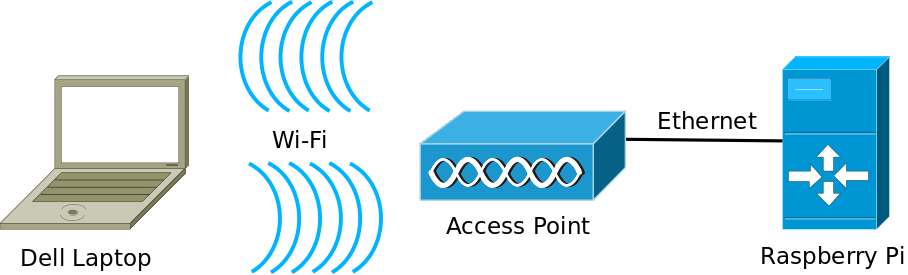
\includegraphics[width=8cm]{Deployment/In_Office_Lab}
	\caption{In-Office Lab Deployment}
	\label{image:In_Office_Lab_Deployment}
\end{figure}

The Pi was the device from which the Pings were sent towards the Laptop. As illustrated in figure \ref{image:In_Office_Lab_Deployment} the Pi and access point were connected via Ethernet. The laptop was connected with the AP via 802.11n. Throughout the tests at the In-lab office we switched between 2.4 and 5.0 GHz band depending on the goal of the experiment. The In-Office lab played a key role to test the features we included in our GoPing tool prior to running experiment at Orbit lab testbed.

\subsection*{Orbit Lab}

The second testbed we worked with was Orbit Lab \cite{orbit2005}. Orbit lab can be considered a large testbed in which different Wireless technologies can be tested. One of these Wireless technologies is 802.11. Within Orbit Lab we worked with Sandbox 4 (SB4) which includes features to vary the attenuation between the nodes in the Sandbox. The main components of SB4 we worked with are the followings.

\begin{enumerate}
	\item SB4 has 9 nodes, each one of them runs Ubuntu 12.04
	\item Attenuation Controller which makes possible to vary the attenuation between the nodes.
\end{enumerate}

Each of the nodes has an Atheros Wireless card, the models are Atheros 5K and 9K. The nodes we worked with have Atheros chipsets which allowed us to collect detailed logs. The links between the nodes in SB4 can be set to attenuation values between 0-30 dBm from the attenuation controller. The topology of SB4 depends on the attenuation values for each link. For example a full-mesh topology is achieved when the attenuation value for all the links is set to 0 dBm. The feature of setting different attenuation values allowed us to test two scenarios associated to WiFi issues. The main deployment we worked with is a replica of the deployment we setup the In-office lab. The node working as AP was setup using the \emph{hostapd} utility. The WLAN settings for the AP are summarized in table \ref{table:WLAN_Settings_AP_Node}.

\begin{table}[h]
	\begin{center}
		\begin{tabular}{||c c||}
			\hline
			Setting & Value\\ [0.5ex] 
			\hline\hline
			802.11 Protocol & 802.11n\\ 
			\hline
			Channel Bonding & No\\
			\hline
			Band & 2.4 GHz\\
			\hline
			Security & Open\\ [1ex] 
			\hline
		\end{tabular}
	\end{center}
\caption{WLAN Settings at AP Node}
\label{table:WLAN_Settings_AP_Node}
\end{table} 


\subsection*{Experiments Setup}

In order to trigger WiFi and non-WiFi issues we setup three main scenarios in Orbit SB4 testbed. Two of them were associated to WiFi issues, attenuation and congestion. The third one was an issue at the access link. Across the three scenarios logging, GoPing, Wireless capture and iPerf measurement are similar. Our experiment sessions lasted for 10 min. During the session we collected Wireless stats logs every 10 secs at the AP and Wireless client. We also setup a Wireless a Sniffer to obtain Over-the-Air packet captures. From the wired client we sent the pings towards the AP and log the stats from GoPing. For the throughput measurement with iPerf, we setup iPerf server at the wireless node and the iPerf client at the wired node. iPerf was setup in TCP mode with 4 parallel TCP streams. We chose TCP as it is transport protocol most commonly used by services at Home WiFi networks. We decided to work with 4 parallel streams as within a Home WiFi the number of TCP in average is below 5 TCP streams \textbf{[We need a reference here]}.

\subsection*{Attenuation}

To trigger attenuation impairments in the testbed we varied the attenuation at the link between the wireless client and the access point. The deployment we worked with derived from the one illustrated in figure \ref{image:In_Office_Lab_Deployment}.  The only additional component is the node working as a wireless sniffer. The attenuation issue was triggered in third and ninth minute of the 10 min session. The experiment was designed this way to set a comparison between non-issue and issue conditions. We setup 5 scenarios with an increase of 3 dBm per impairment interval. Table \ref{table:Attenuation_Experiment_Values} breakdowns the scenarios and the attenuation levels for each impairment interval. Each one of the experiments was run 5 times.

\begin{table}[h!]
	\begin{center}
		\begin{tabular}{|| m{5em} | m{2cm}| m{2cm} ||}
			\hline
			\multirow{2}{*}{Scenario} & \multicolumn{2}{c||}{Attenuation Value {[}dBm{]}} \\ \cline{2-3} 
			& \multicolumn{1}{l|}{1st Interval} & \multicolumn{1}{l||}{2nd Interval} \\ \hline\hline
			1 & 3 & 6 \\ \hline
			2 & 9 & 12 \\ \hline
			3 & 15 & 18 \\ \hline
			4 & 21 & 24 \\ \hline
			5 & 27 & 30 \\ \hline
		\end{tabular}
	\end{center}
	\caption{Attenuation Scenarios and Values}
	\label{table:Attenuation_Experiment_Values}
\end{table}

\subsection*{Congestion}

To trigger congestion in our testbed, we connected more wireless nodes to the same AP our main wireless client was connecting to. At the 4th and 8th minute we connected an additional wireless node to the AP. The additional wireless node client sent iPerf UDP traffic to the AP, hence the AP was running an iPerf server instance. We increased by one the wireless nodes connected to the AP by one per issue interval. Table \ref{table:Congestion_Experiment_Values} consolidates the scenarios and number of wireless nodes connected to the AP.

\begin{table}[h!]
	\begin{center}
		\begin{tabular}{|| m{5em} | m{2cm}| m{2cm} ||}
			\hline
			\multirow{2}{*}{Scenario} & \multicolumn{2}{l||}{Connected Wireless Nodes} \\ \cline{2-3} 
			& \multicolumn{1}{l|}{1st Interval} & \multicolumn{1}{l||}{2nd Interval} \\ \hline\hline
			1 & 1 & 1 \\ \hline
			2 & 2 & 2 \\ \hline
			3 & 3 & 3 \\ \hline
			4 & 4 & 4 \\ \hline
			5 & 5 & 5 \\ \hline
		\end{tabular}
	\end{center}
	\caption{Congestion Scenarios and Values}
	\label{table:Congestion_Experiment_Values}
\end{table}

\subsection*{Access Link Limiting}

The third scenario experimented in the testbed was a non-WiFi issue. The issue consisted in limiting the access link capacity at the Wired node. We achieved limiting at the wired node by using \emph{tc} which is a traffic shaper. In a similar way to the attenuation scenario, we triggered the issue at the 3rd and 9th minute of the 10 min experiment window. Table \ref{table:Access_Link_Experiment_Values} details the scenarios and values used for the Access Link Limiting scenario.

\begin{table}[h!]
	\begin{center}
		\begin{tabular}{|| m{5em} | m{2cm}| m{2cm} ||}
			\hline
			\multirow{2}{*}{Scenario} & \multicolumn{2}{c||}{Throughput {[}Mbps{]}} \\ \cline{2-3} 
			& \multicolumn{1}{l|}{1st Interval} & \multicolumn{1}{l||}{2nd Interval} \\ \hline\hline
			1 & 100 & 90 \\ \hline
			2 & 80 & 70 \\ \hline
			3 & 60 & 50 \\ \hline
			4 & 40 & 30 \\ \hline
			5 & 20 & 10 \\ \hline
		\end{tabular}
	\end{center}
	\caption{Access Link Limiting Scenarios and Values}
	\label{table:Access_Link_Experiment_Values}
\end{table}

\begin{itemize}
	\item \textbf{Attenuation}
	\begin{itemize}
		\item We have been using the embedded manger for attenuation in Orbit.
		\item We can instrument attenuation values on the links connecting the nodes, in our case we vary the attenuation values between Wireless client and AP.
		\item Attenuation controller allows to define values in the range from 0 - 30 dBm.
		\item For our experiment we have been varying the values from 0 to 30 in steps of 3.
		\item We vary the attenuation and record the RTTs for pings.
		\item We have identified that after 27 dBm of attenuation is when we begin to see an increase in RTTs, each session last 10 min. Probe rate every 200msec.
		\item At 30 dBm the connectivity between Wireless client and AP is lost.
		\item For bandwidth test we have run iPerf and recorded the bandwidth obtained at the client side.
		\item \textbf{With 5GHz we identified that after 6dBm the connectivity between client and AP is lost.}
		\item We have setup 802.11n using 2.4GHz band to increase the range.
		\item The goal is to run iPerf and identify at which attenuation levels does the bitrates drops, record the attenuation values to run ping tests.
		\item Once the attenuation values have been identified the next step is to run ping tests using the attenuation values found with iPerf test and record the average RTTs.
		
	\end{itemize}


\textbf{Main ideas for Orbit test bed description}

\begin{enumerate}
	\item Orbit is a testbed mostly devoted to Wireless experiments. (Mostly as they also have SDN sandboxes to test SDN technologies)
	\item We have been using the Sandbox 4, SB4, which is devoted to Wi-Fi and Wi-Max Experiments.
	\item SB4 is made of 9 nodes, each of them runs Linux based systems, Ubuntu 12.04 to be precise.
	\item Our main setup is composed by three nodes. One node plays the role of the AP, another the role of Wireless client and the last one is a Wired client.
	\item We are using 802.11n in 2.4GHz band to improve the reachability of the AP and the Wireless client.
	\item The wired client is the source of the probes and iPerf server.
	\item Wireless client plays the role of iPerf client.
	\item We can include a diagram of the Orbit SB4 deployment and include the proper references.
\end{enumerate}

\textbf{Main ideas for the evaluation methods}



	%\item \textbf{Wi-Fi Interference}
	%\begin{itemize}
	%	\item To create Wi-Fi interference we will deploy a 2nd Wireless client and 2nd AP.
	%	\item These two nodes will be set to operate in the same channel as the first Wireless client and AP.
	%	\item The goal is to create an interference in which the source of the interference speaks Wi-Fi, meaning it can request time transmit, wait for the other station to transmit and transmit.
	%\end{itemize}
	
	\item \textbf{Interference}
	\begin{itemize}
		\item Currently looking for a way to create Noise in SB4.
		\item Check if for a specific time they can setup a Microwave oven or similar.
		
	\end{itemize}
	
	
	
	\item Congestion
	\begin{itemize}
		\item For this experiment we will deploy a second wireless client connected to the same AP.
		\item The 2nd Wireless client will send traffic to the iPerf server located in the wired client.
		\item The original client will continue to send pings to the wired client.
		\item We will record the results of RTT while other client is sending traffic to the iPerf Server.
		
	\end{itemize}
	
	
\end{itemize}


We used three nodes with.
Atheros 9k and 5k wireless cards.

We configure a node to work as a Wireless station, another as an AP and finally a third one as a wired client from where the pings were issued.

The third node working as a wired client plays a similar role as the Pi in our In-lab setup.


\subsection{Setup of testbed}

Here we explain how we ran the experiments.

\subsection{RSSI in the wild}

In order to collect realistic metric from can be considered a common value of RSSI in the wild we ran survey to collect this metric. We asked our colleagues in our office to run a script from which's output we can extract the RSSI value. We obtained ~760 samples metrics coming from different environment contexts,  mainly home and offices. We found RSSI average value in the wild to range between -60 and -60 [dBm]. Following picture depicts the histogram of RSSI obtained from the survey.

\begin{figure}[h]
	\centering
	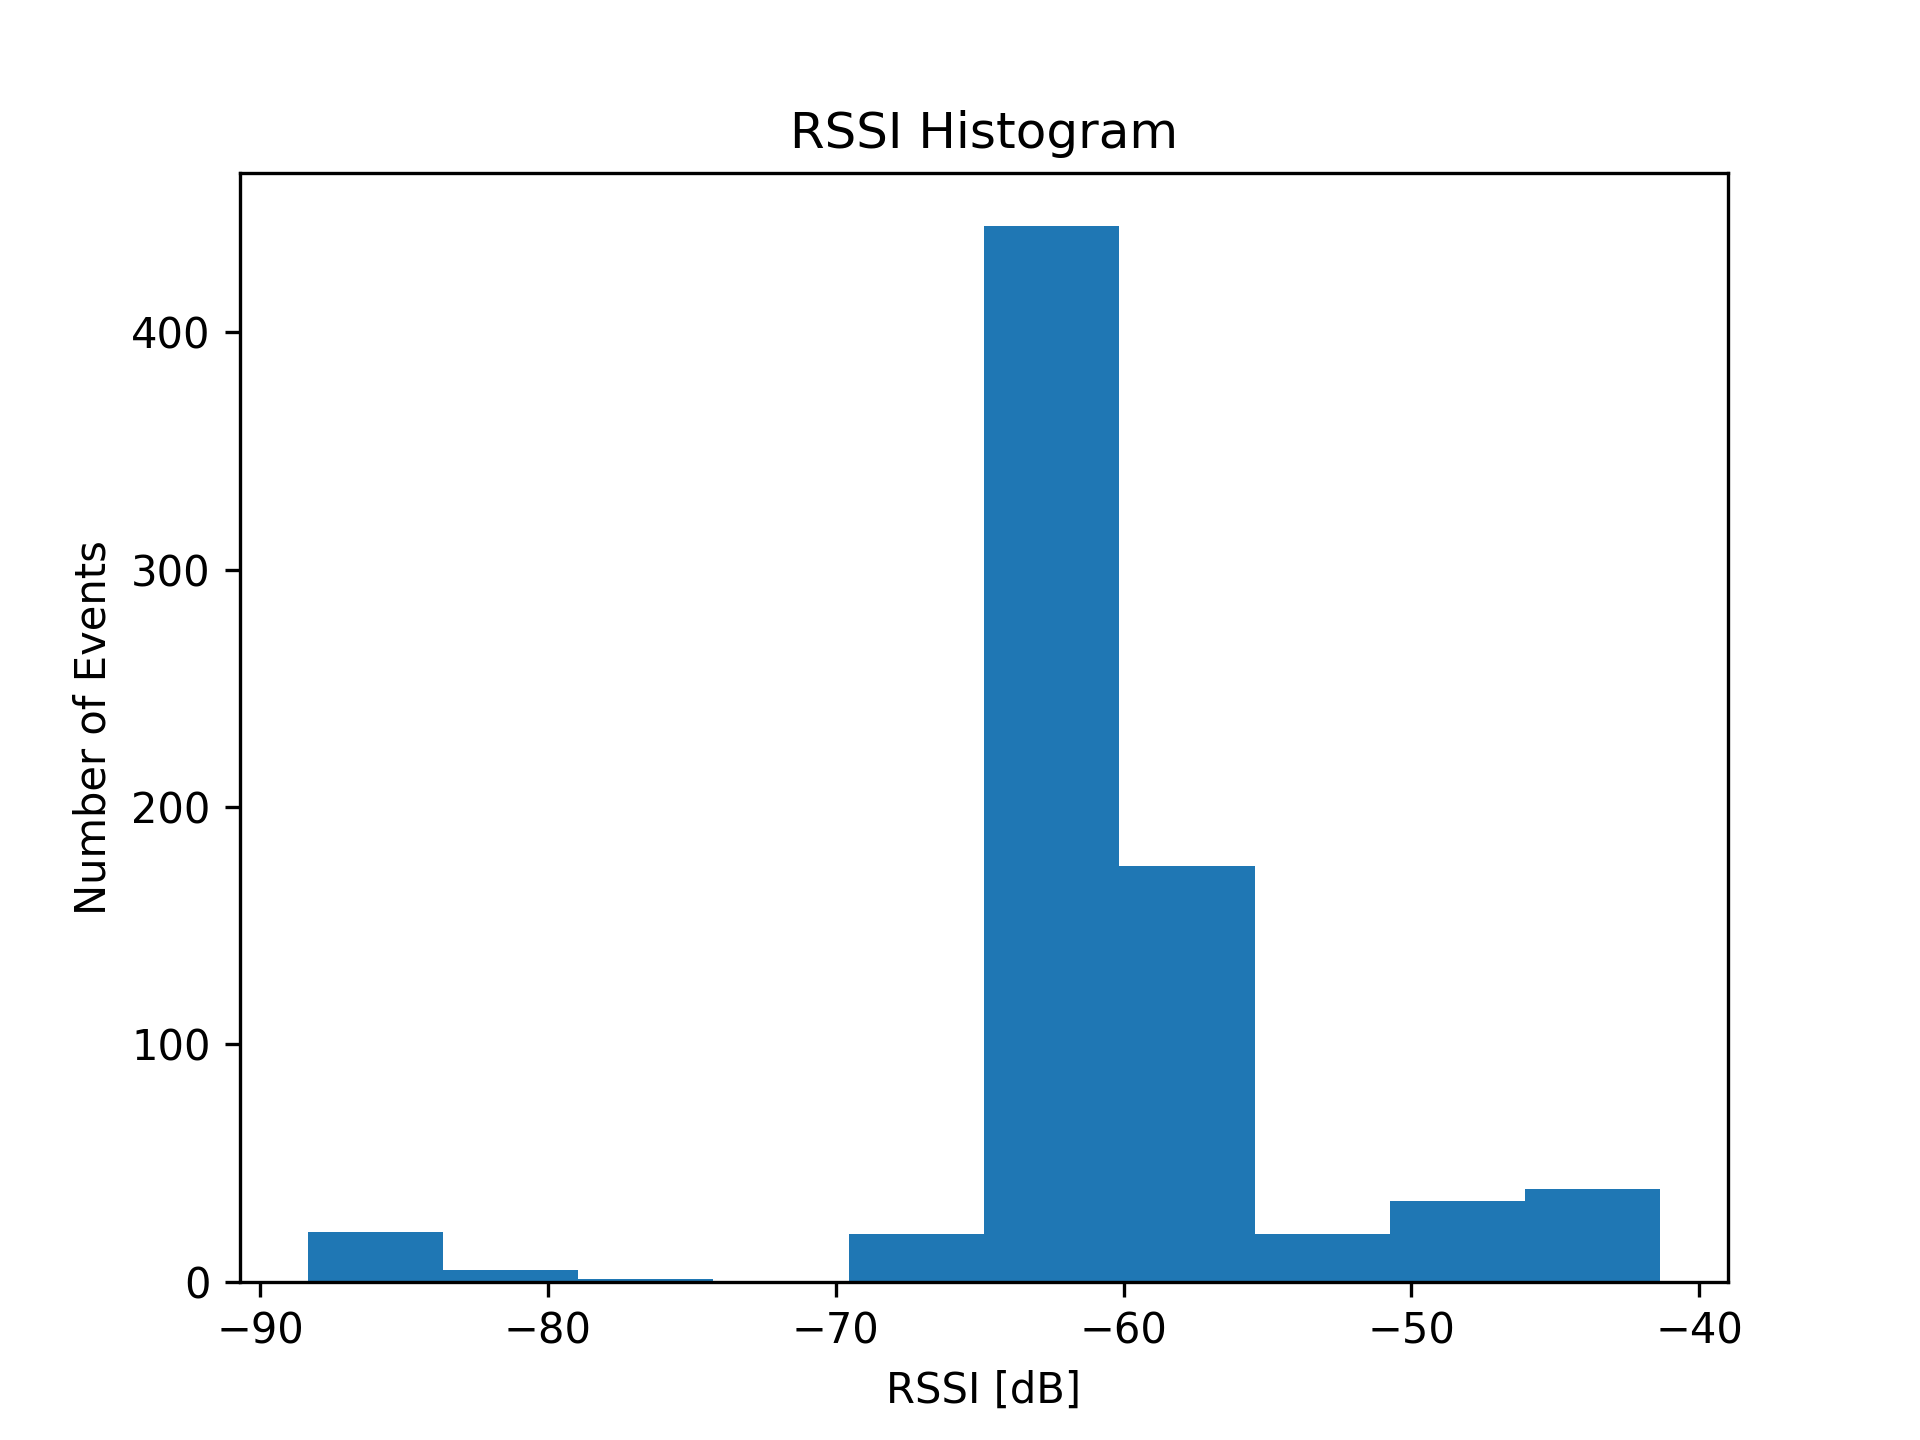
\includegraphics[width=8cm]{RSSI_Stats/RSSI_Histogram}
	\caption{RSSI Survey Values Histogram}
	\label{fig:vSDN_Controller_DC}
\end{figure}


The main goal of this exercise is setup our testbed attenuation settings to trigger an RSSI value similar to the one found with the survey. In our testbed the attenuation values which lead to an RSSI value between the found range are 0, 3 and 6 [dBm] in the 2.4 GHz band.


We can include the accuracy of our methods depending on where are we setting our Vantage point.ex

In our lab we placed the laptop and the Pi close to each other, a distance smaller than 5 m. We connected to the 5GHz band under 802.11n protocol.

The first set of experiments consisted in progressively adding TCP sessions. The goal was to perceive how was RTT changed with more TCP sessions. We expected to see an increase as more TCP session were added.

Results matched our expectation and saw an increase in average RTT as more TCP session were added.

\textbf{Include plot in which we have the CDF of RTTs vs TCP Streams}

The next set of experiments were ran with the goal of finding a suitable probing rate. The ideal case is to probe frequent enough to have a "good" sense of the network without adding overhead and disrupting the Wireless Network.

We issued pings in sessions of 10 min at a ping rate of 100msec, initially, we call this aggressive scenario. The rate was defined to be 100msec to set our baseline from which we derived our sampling to obtain a suitable probing rate. The main goal is to achieve a rate which is not as aggressive as probing every 100msec.

After completing our sample analysis, we define it to be 200msec and we proceed to run test in Orbit where we can modify parameters as attenuation.

Orbit lab allow to modify attenuation from 0 dB to 30 dB. We perceived an increase in average RTT and loss rate from 27dB to 29dB. (At 30 dB link is unusable).

The results are show in the following plots.

\textbf{Include Plots with Avg RTTs and Loss Rate results from Orbit}




